\documentclass[12pt,a4paper]{article}

\usepackage[utf8]{inputenc}
\usepackage[T1]{fontenc}
\usepackage[english]{babel}
\usepackage[margin=2cm]{geometry}
\usepackage{times}
\usepackage{setspace}
\setstretch{1.15}
\usepackage{graphicx}
\usepackage{float}
\usepackage{booktabs}
\usepackage{amsmath,amssymb}
\usepackage{array}
\usepackage[hidelinks]{hyperref}
\usepackage{fancyhdr}

\pagestyle{fancy}
\fancyhf{}
\fancyfoot[C]{\thepage}
\renewcommand{\headrulewidth}{0pt}
\renewcommand{\footrulewidth}{0pt}

\begin{document}

\begin{titlepage}
    \centering
    \vspace*{3cm}
    {\Huge \bfseries Report 8}\\[0.5cm]
    {\large Course: Introduction to Drone Technology}\\[3cm]
    \textbf{\Large Participating Students:}\\[0.8cm]
    \begin{tabular}{ll}
        \textbf{Full Name 1:} & Luka Rizman (luriz26@student.sdu.dk) \\
        \textbf{Full Name 2:} & Matic Kern (maker26@student.sdu.dk) \\
        \textbf{Full Name 3:} & Adrian Maslak (admas26@student.sdu.dk) \\
    \end{tabular}
    \vfill
    {\large \textbf{Date:} \today}
    \vspace*{1.5cm}
\end{titlepage}

\clearpage
\pagenumbering{arabic}

\par\medskip
\noindent\textbf{3}\quad\textbf{Exercises}

\par\medskip
\noindent\textbf{3.1}\quad\textbf{Antenna construction}

\par\medskip
\noindent\textbf{Construction parameters}

The antenna was constructed as a half-wave dipole for the target resonant
frequency of $434\,\mathrm{MHz}$. The dipole was made from PVC-insulated
electrical wire and mounted straight along a wooden dowel.

\begin{table}[H]
    \centering
    \begin{tabular}{>{\raggedright\arraybackslash}p{0.48\textwidth}p{0.4\textwidth}}
        \toprule
        \textbf{Parameter} & \textbf{Value / notes} \\
        \midrule
        Target resonant frequency & $434\,\mathrm{MHz}$ \\
        Conductor & PVC-insulated electrical wire \\
        Initial length of radial 1 & $190\,\mathrm{mm}$ \\
        Initial length of radial 2 & $190\,\mathrm{mm}$ \\
        Total initial tip-to-tip length & $380\,\mathrm{mm}$ \\
        Mounting & Wooden dowel and electrical tape \\
        \bottomrule
    \end{tabular}
    \caption{Construction parameters of the dipole antenna.}
\end{table}

The coaxial cable was prepared by stripping approximately $5$--$7\,\mathrm{mm}$
of the outer jacket. The braid was folded back and soldered to radial 2,
while the centre conductor was soldered to radial 1. Continuity and the
absence of a short circuit between the radials were checked with a Keysight
U1231A multimeter. The coaxial cable was routed perpendicular to the dipole
with a gentle bend radius.

\par\medskip
\noindent\textbf{Required photo}

\begin{figure}[H]
    \centering
    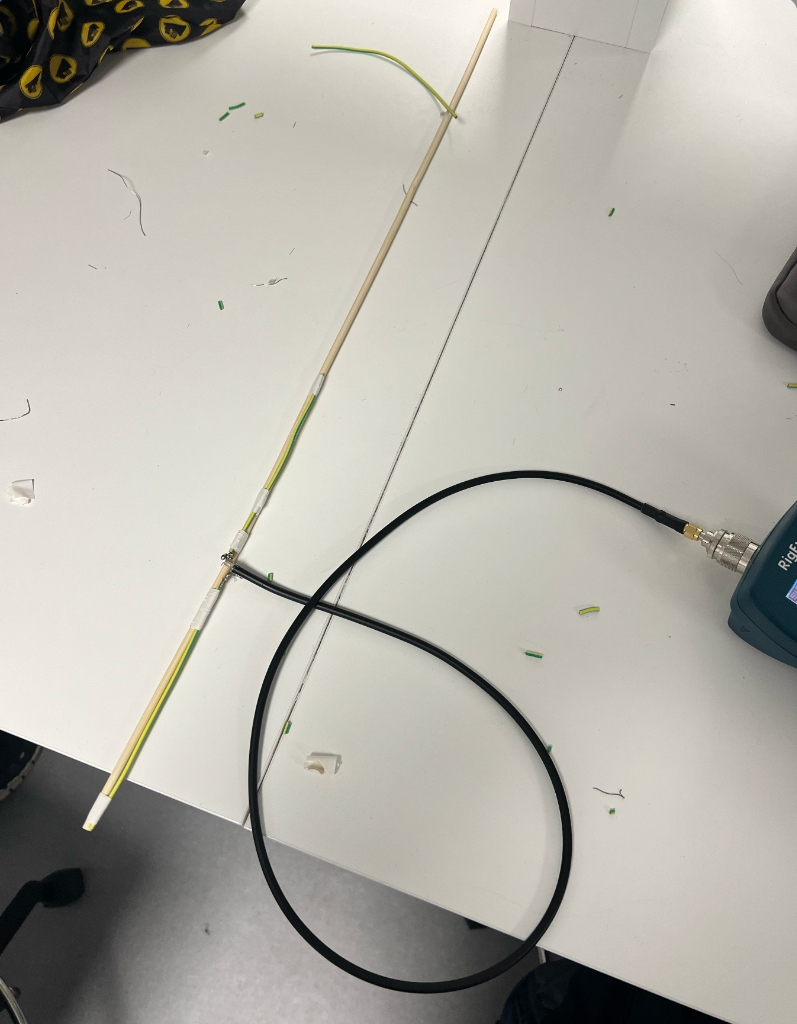
\includegraphics[width=0.65\textwidth]{images/antenna_final.jpg}
    \caption{Constructed and tuned $434\,\mathrm{MHz}$ half-wave dipole antenna.}
    \label{fig:antenna}
\end{figure}

\par\medskip
\noindent\textbf{3.2}\quad\textbf{Antenna tuning (RigExpert)}

\par\medskip
\noindent\textbf{Iterative tuning log}

\begin{table}[H]
    \centering
    \scriptsize
    \begin{tabular}{c c c c c c c}
        \toprule
        \textbf{Step} & \textbf{Trim (mm)} & \textbf{Lengths (mm)}
        & \textbf{Range} & \textbf{$f_r$ (MHz)} & \textbf{Min SWR}
        & \textbf{SWR at 434 MHz} \\
        \midrule
        0 & 0 & 190/190 & $\pm100$ MHz & 340 & 1.40 & 7.00 \\
        1 & 10 & 180/180 & $\pm100$ MHz & 366 & 1.13 & 5.50 \\
        2 & 10 & 170/170 & $\pm100$ MHz & 391 & 1.15 & 4.00 \\
        3 & 5 & 165/165 & $\pm50$ MHz & 400 & 1.18 & 3.00 \\
        4 & 6 & 159/159 & $\pm50$ MHz & 411 & 1.28 & 2.50 \\
        5 & 5 & 154/154 & $\pm25$ MHz & 426.5 & 1.28 & 1.40 \\
        6 & 2 & 152/152 & $\pm25$ MHz & 437 & 1.23 & 1.33 \\
        Final & 0 & 152/152 & $\pm25$ MHz & 433 & 1.15 & 1.18 \\
        \bottomrule
    \end{tabular}
    \caption{SWR tuning measurements.}
\end{table}

\par\medskip
\noindent\textbf{Final tuned antenna summary}

The final radial lengths were $152\,\mathrm{mm}/152\,\mathrm{mm}$, resulting
in a total physical dipole length of $304\,\mathrm{mm}$. The measured
resonant frequency was approximately $433\,\mathrm{MHz}$ and the SWR at
$434\,\mathrm{MHz}$ was approximately $1.18:1$.

The empirical shortening factor is
\[
    \frac{L_{\mathrm{phys}}}{\lambda/2}
    = \frac{304}{345.6} \approx 0.880.
\]
The reflected power ratio at $S=1.18$ is
\[
    \frac{P_r}{P_f}
    = \left(\frac{S-1}{S+1}\right)^2
    \approx 0.00682,
\]
which corresponds to approximately $0.68\%$ reflected power and
$99.32\%$ transmitted power. The mismatch loss is approximately
$-0.03\,\mathrm{dB}$.

\begin{figure}[H]
    \centering
    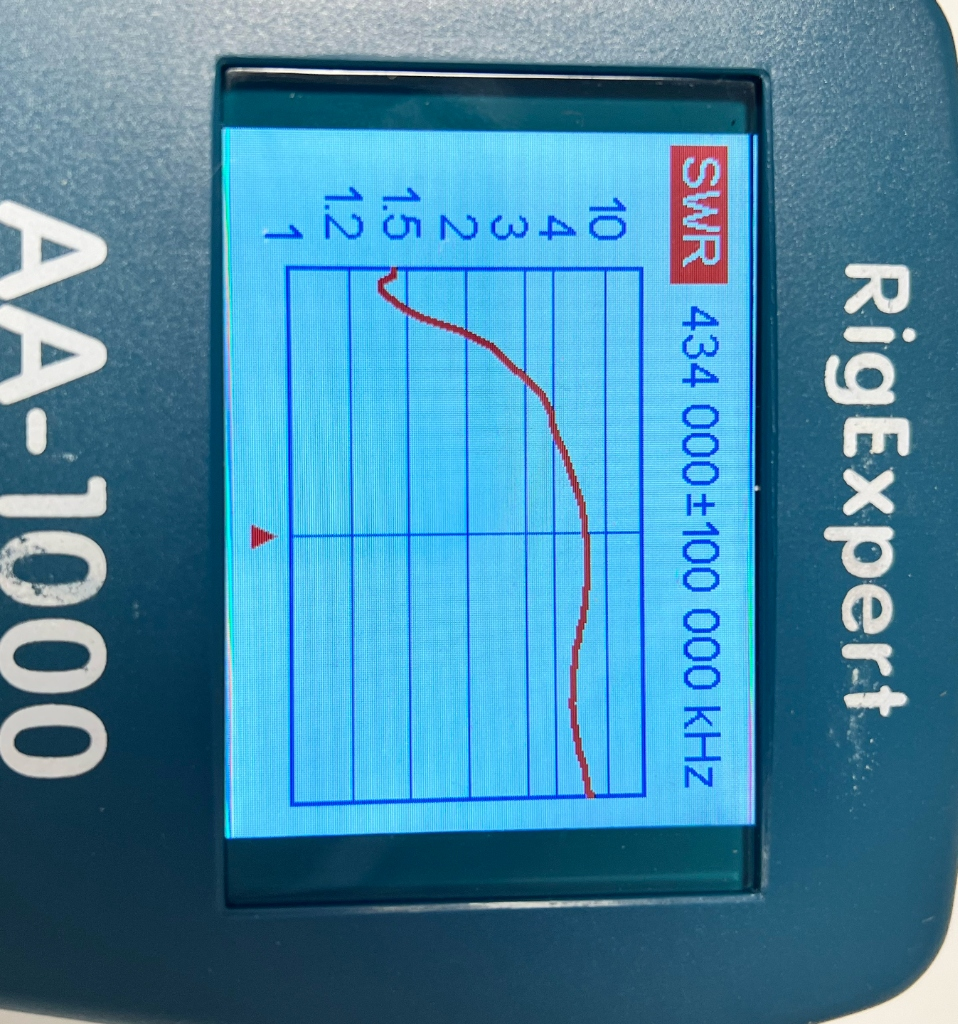
\includegraphics[width=0.8\textwidth]{images/swr_scan_0_initial.jpg}
    \caption{Initial SWR scan.}
    \label{fig:swr-initial}
\end{figure}

\begin{figure}[H]
    \centering
    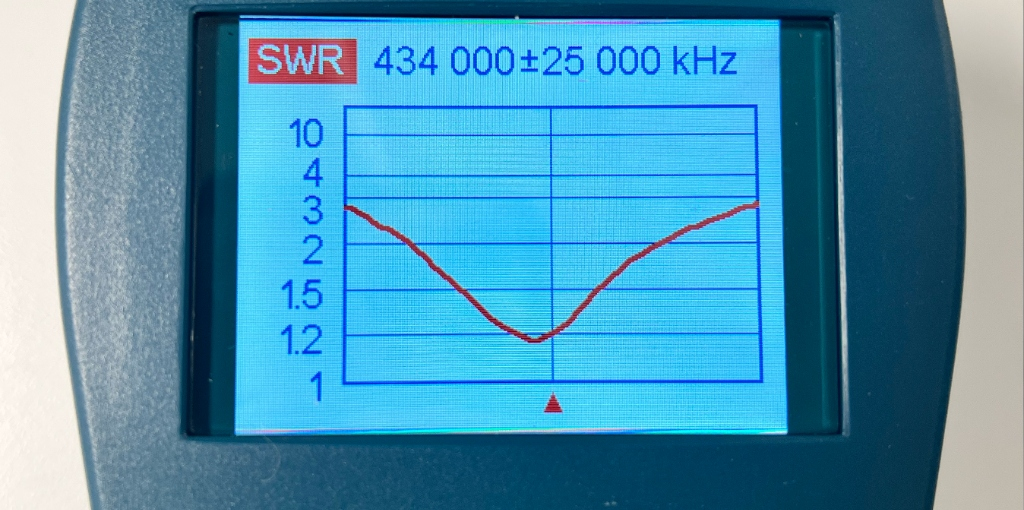
\includegraphics[width=0.8\textwidth]{images/swr_scan_final_434mhz.jpg}
    \caption{Final SWR scan centred around $434\,\mathrm{MHz}$.}
    \label{fig:swr-final}
\end{figure}

\par\medskip
\noindent\textbf{3.3}\quad\textbf{Antenna near-field obstacles}

\par\medskip
\noindent\textbf{Q1: Hand approaching along the coax}

As the hand approached the antenna, the SWR increased and the resonance dip
became broader. The minimum SWR changed from approximately $1.15$ in the
free-hanging case to approximately $1.62$ at a distance of about $20\,\mathrm{cm}$.

\par\medskip
\noindent\textbf{Q2: Change in resonant frequency}

The resonant frequency shifted downwards as the hand approached. It changed
from approximately $433\,\mathrm{MHz}$ in the baseline measurement to
approximately $431\,\mathrm{MHz}$ at $35\,\mathrm{cm}$ and
$426$--$427\,\mathrm{MHz}$ at $20\,\mathrm{cm}$. The hand adds capacitive
loading and increases the effective electrical length.

\par\medskip
\noindent\textbf{Q3: Conducting obstacles at various distances}

\begin{table}[H]
    \centering
    \begin{tabular}{p{0.32\textwidth}p{0.13\textwidth}p{0.2\textwidth}p{0.2\textwidth}}
        \toprule
        \textbf{Obstacle} & \textbf{Distance} & \textbf{Effect on $f_r$}
        & \textbf{Effect on SWR} \\
        \midrule
        Metal chair, strong coupling & $15\,\mathrm{cm}$ & $\approx413\,\mathrm{MHz}$
        & SWR at 434 MHz $\approx2.2$ \\
        Metal chair, moderate coupling & $15\,\mathrm{cm}$ & $\approx432\,\mathrm{MHz}$
        & Minimum SWR $\approx1.55$ \\
        \bottomrule
    \end{tabular}
    \caption{Influence of conducting obstacles.}
\end{table}

Conducting obstacles couple electromagnetically to the antenna and alter its
radiation resistance and reactance. This causes detuning and an increase in
SWR.

\par\medskip
\noindent\textbf{Q4: Sensitivity to obstacle angles}

The antenna is most sensitive to obstacles at $90^\circ$ to the dipole axis,
where the radiation field is strongest. It is least sensitive along the
dipole axis, where a half-wave dipole has radiation nulls. In the reactive
near field, however, objects close to the radial tips can still cause strong
capacitive detuning.

\par\medskip
\noindent\textbf{3.4}\quad\textbf{Outdoor range test}

\par\medskip
\noindent\textbf{Test setup and logging configuration}

The outdoor test should be performed in a clear line-of-sight environment.
The antenna polarization and orientation must remain the same for the
reference and custom-antenna measurements. The ground station and drone
telemetry modems should be logged using the ROS2 scripts
\texttt{log\_global\_pos.py} and \texttt{log\_radio\_rssi.py}.

\begin{table}[H]
    \centering
    \begin{tabular}{p{0.45\textwidth}p{0.4\textwidth}}
        \toprule
        \textbf{Parameter} & \textbf{Value} \\
        \midrule
        Test location & To be filled in \\
        Weather / environment & To be filled in \\
        Telemetry modem TX power & To be filled in \\
        Antenna polarization / orientation & To be filled in \\
        Logging scripts & \texttt{log\_global\_pos.py}, \texttt{log\_radio\_rssi.py} \\
        \bottomrule
    \end{tabular}
    \caption{Outdoor range-test setup.}
\end{table}

\par\medskip
\noindent\textbf{Range test measurements summary}

\begin{table}[H]
    \centering
    \begin{tabular}{p{0.4\textwidth}p{0.2\textwidth}p{0.2\textwidth}}
        \toprule
        \textbf{Configuration} & \textbf{Maximum distance (m)}
        & \textbf{RSSI trend} \\
        \midrule
        Reference antennas & To be filled in & To be filled in \\
        Custom $434\,\mathrm{MHz}$ dipole & To be filled in & To be filled in \\
        \bottomrule
    \end{tabular}
    \caption{Outdoor range-test measurements.}
\end{table}

\par\medskip
\noindent\textbf{Required photos and plots}

\begin{itemize}
    \item Outdoor test scenario.
    \item Reference antennas: RSSI versus distance.
    \item Custom dipole antenna: RSSI versus distance.
    \item Direct comparison of reference and custom antenna results.
\end{itemize}

\par\medskip
\noindent\textbf{Q5: Antenna gain compared to the issued antennas}

The relative gain should be estimated from the RSSI difference at equivalent
distances in the clear line-of-sight region. The result can be cross-checked
using
\[
    \Delta G = 20\log_{10}\left(\frac{d_{\mathrm{dipole}}}
    {d_{\mathrm{reference}}}\right).
\]
The measured values and the calculated gain should be added after the outdoor
range test.

\end{document}
